\documentclass{report}
\usepackage{amsthm,amsmath,amssymb}
\usepackage{tikz}
\usetikzlibrary{intersections}

\begin{document}
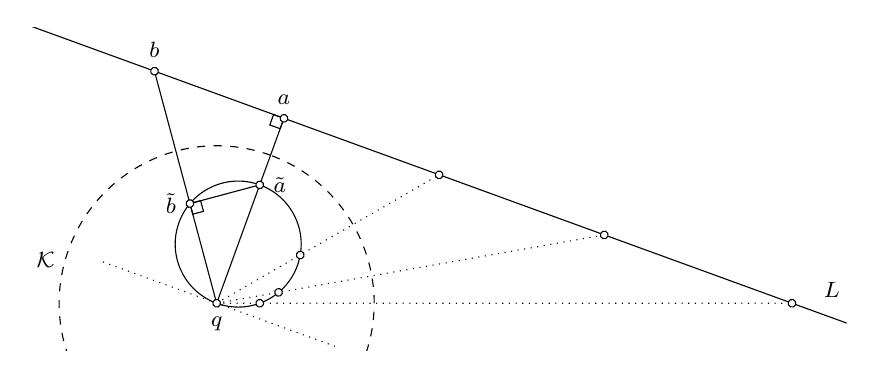
\begin{tikzpicture}[scale=2]\footnotesize
  \clip (-1.2,-.3) rectangle (4,1.75);
  \begin{scope}[rotate=70]
    \coordinate (q) at (0,0);
    %
    \draw[dashed] (q) circle (1);
    \draw[dotted](0,-.8)--(0,.8)node[left=1.5em]{$\mathcal{K}$};
    %
    \path[name path=ray1] (q)-- (35:3cm);
    \path[name path=ray2] (q)-- (0:3cm);
    \path[name path=ray3] (q)-- (-40:3cm);
    \path[name path=ray4] (q)-- (-60:3.5cm);
    \path[name path=ray5] (q)-- (-70:4cm);
    \draw[name path=circulo] (q)+(.4,0) circle (.4);
    \draw[name path=vertical] (1.25,-4)node[above left=10pt]{$L$} -- (1.25,2);
    %
    \draw[name intersections={of=ray1 and vertical,by={b}}]  (q)--(b);
    \draw[name intersections={of=ray2 and vertical,by={a}}]  (q)--(a);
    \draw[dotted,name intersections={of=ray3 and vertical,by={v3}}]  (q)--(v3);
    \draw[dotted,name intersections={of=ray4 and vertical,by={v4}}]  (q)--(v4);
    \draw[dotted,name intersections={of=ray5 and vertical,by={v5}}]  (q)--(v5);
    %
    \path[name intersections={of=ray1 and circulo,by={btilde}}] ;
    \path[name intersections={of=ray2 and circulo,by={atilde}}] ;
    \path[name intersections={of=ray3 and circulo,by={c31,c32}}] ;
    \path[name intersections={of=ray4 and circulo,by={c41,c42}}] ;
    \path[name intersections={of=ray5 and circulo,by={c51,c52}}] ;
    %
    \draw (atilde)--(btilde);
    \draw[rotate=35] (btilde) rectangle +(-.07,-.07);
    \draw[rotate=0] (a) rectangle +(-.07,.07);
    \foreach \p in {q,btilde,atilde,c32,c42,c52,b,a,v3,v4,v5}{
      \draw[fill=white] (\p) circle (.7pt); 
    }
    %
    \node[left=2pt] at (btilde){$\tilde b$};
    \node[right=2pt] at (atilde){$\tilde a$};
    \node[above=2pt] at (a){$a$};
    \node[above=2pt] at (b){$b$};
    \node[below=2pt] at (q){$q$};
  \end{scope}
\end{tikzpicture}
\end{document}
